%Základní metody úpravy a segmentace obrazu (filtrace, prahování, hrany).

\subsection{Prahování}
\begin{itemize}
	\item Cílem práhování je \textbf{oddělit pozadí od popředí} na základně stanoveného prahu (nějaká realná hodnota). Výsledkem binární obraz (1 = objekt, 0 = pozadí).
	\item Práh může být buď \textbf{stejný} pro celý obrázek, anebo \textbf{adaptivní} pro jednotlivé části obrazu. Další možností je stanovit práh v \textbf{intervalu} $<a, b>$. Úspěšnost detekci oblastí závisí na správné hodnotě prahu.
	\item Pokud neznáme hodnotu prahu, snažíme se jí stanovit na základně informací získaných z obrazu, který má být \textbf{segmentovaný}.
	\item \textbf{Bimodální histogra}m (dva kopce), \textbf{multimodální histogram }-- práh určit jako \textbf{minimum histogramu} mezi vysokými hodnotami, pak lze dále rekurzivně dělit (předpokládáme, že v obraze jsou převážně dva a více druhů pixelů).
	\item \textbf{Obraz lze rekurzivně dělit} na menší části, ve kterých se vypočte histogram a dle něho určí práh pro konkrétní část (pokud nelze práh určit, lze ho interpolovat pomocí sousedních prahů).
	\item \textbf{Minimalizace rizika chyby}:
	\begin{itemize}
		\item stanovení prahu tak, aby se minimalizovala špatná detekce,
		\item stanovení dle aproximace normálních rozdělení popředí a pozadí \\$\varepsilon = \theta P(t) + (1 - \theta)[1 - Q(t)]$.
		\item nejlepších výsledků lze dosáhnout v \textbf{extrému první derivace}
		\item pokud je zastoupení pozadí a popředí stejné a má stejný rozptyl $(t - \mu )^2 = (t - v)^2 $.
	\end{itemize}
	\begin{figure}[H]
\centering
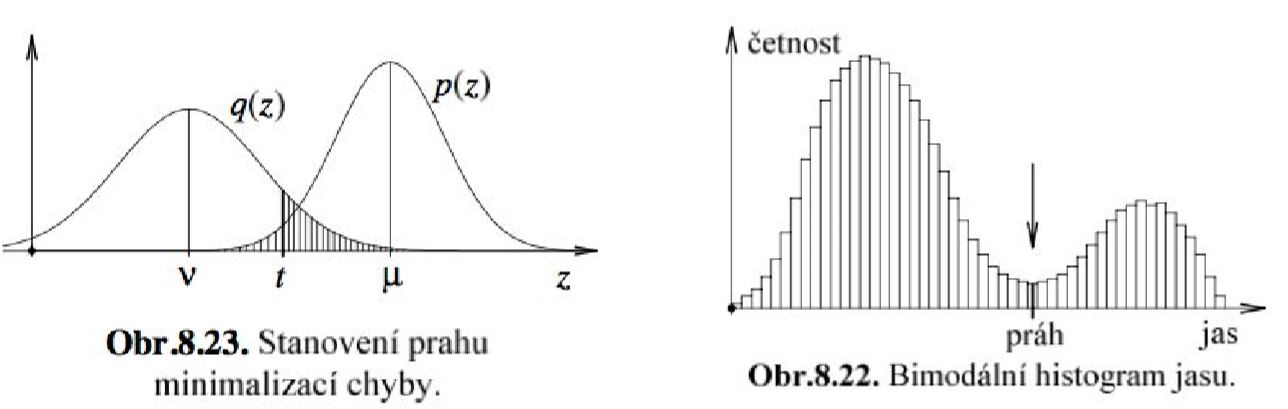
\includegraphics[width=0.8\textwidth]{assets/8_prah_histogram}
\end{figure}
\item Na levém obrázku je prah označen $t$ a vyšrafovaná oblast značí chybu, která nastane při prahování, kdy bude špatně rozpoznané popředí/objekt $q(z)$ a pozadí $p(z)$ -- minimalizace chyby. 
\end{itemize}


\subsection{Detekce hran}
\begin{itemize}
	\item Každá oblast je obklopena hranicí.
	\item Hranice se skládá z hran (případně také z jediné zakřivené hrany).

	\item Hrana se skládá z jednotlivých hranových bodů.
	\item Většinou se postupuje tak, že se obraz převede do stupně šedi a následně se naleznou jednotlivé body hran.
	\item Za bod hrany se často považuje místo, kde průběh jasu \textbf{vykazuje náhlou změnu}, případně \textbf{inflexní bod}.
	\item Po nalezení jsou jednotlivé nalezené body hran spojovány různými technikami do hran a celých hranic.
\end{itemize}
\subsubsection{Detekce hran s využitím gradientu}
\begin{itemize}
 	\item Hrana je v obrazu zastoupeny (prudkou) \textbf{změnou jasu}, lze ji tedy najít zkoumáním síly a směru gradientu v jednotlivých bodech.
 	\item Pro určení směru gradientu či hrany (​\textbf{směr gradientu je kolmý ke směru hrany​}) je třeba provést ​ \textbf{derivaci​} (nejlépe v x i y), která je při výpočtu nahrazena diferencí.
 	\item Diference může být buď \textbf{centrální} nebo \textbf{dopředná}/\textbf{zpětná}.
 	\begin{equation*}
 		\begin{split}
 		d_x = \dfrac{I(x - 1, y) - I(x + 1, y)}{2} \, , \quad 		d_y= \dfrac{I(x, y - 1) - I(x, y + 1)}{2} \, .
 		\end{split}
 	\end{equation*}
 	 \item Velikost hrany lze určit velikostí gradientu (norma), hrana je tam, kde $e > \textrm{práh}$. (hrana je kolmá k gradientu) \\
 	 $ e(x, y) = \sqrt{(f_x(x,y)^2+ f_y(x,y)^2})$
 	 \item Směr hrany a gradientu lze určit (kde $\varphi$ -- směr gradientu, $\psi$ -- směr hrany) 
 	  	\begin{equation*}
 		\begin{array}{c}
 		\varphi(x, y) = \arctan{[\frac{f_y(x,y)}{f_x(x,y)}]}, \psi(x,y) = \varphi(x,y) + \frac{\pi}{2}.
 		\end{array}
 	\end{equation*}
 	\item Výše uvedené derivace lze nahradit \textbf{konvolučními maskami}
 	\begin{itemize}
 		\item \textbf{Sobel} -- vážený průměr (Prewittove dělá pouze normální)
 		\item \textbf{Kirsch} -- počítání hran v 8 směrech
 	\end{itemize}
	\item Robertsův operátor:
	\begin{equation*}
 		\begin{bmatrix}
     -1 & 0      \\[0.3em]
     0 & 1  
          \end{bmatrix}.
\end{equation*}
	\item operátor Previttové:
	\begin{equation*}
	 \begin{bmatrix}
     -1 & -1  & -1      \\[0.3em]
      0 &  0  &  0      \\[0.3em]
      1 &  2  &  1      \\
     \end{bmatrix}.
\end{equation*}
	\item Sobelův operátor:
	\begin{equation*}
	 \begin{bmatrix}
     -1 & -2  & -1      \\[0.3em]
      0 &  0  &  0      \\[0.3em]
      1 &  2  &  1      \\
     \end{bmatrix}.
\end{equation*}
	\item Kirschův operátor:
		\begin{equation*}
	 \begin{bmatrix}
     -5 & -5  & -5      \\[0.3em]
      3 &  0  &  3      \\[0.3em]
      3 &  3  &  3      \\
     \end{bmatrix}.
\end{equation*}
\end{itemize}
 		\begin{figure}[H]
 	\begin{center}
	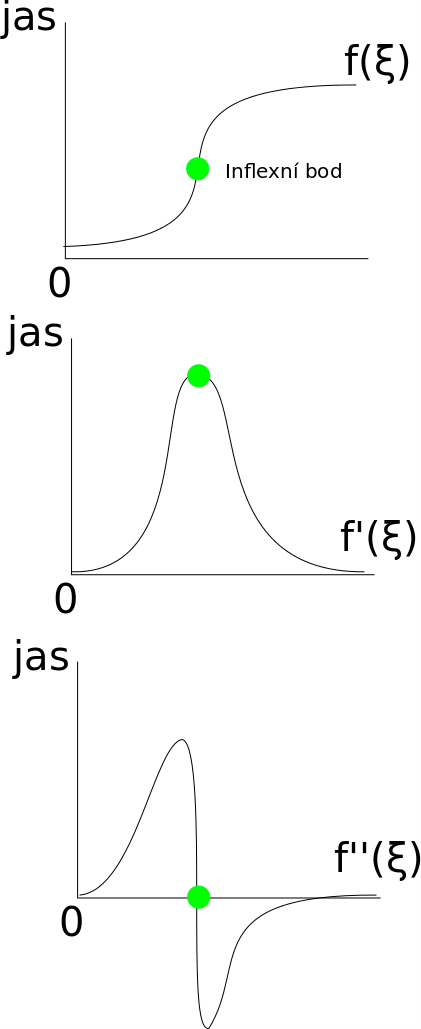
\includegraphics[width=0.25\textwidth]{assets/8_det_hran_grad}
	\caption{Velikost gradientu a jeho první a druhá derivace}
	\end{center}
	\end{figure}
\subsubsection{Detekce hran hledáním průchodu nulou}
\begin{itemize}
	\item První derivace obrazové funkce nabývá svého maxima v místě hrany.
	\item \textbf{Druhá derivace protíná} v místě hrany \textbf{nulovou hodnotu}.
	\item Spolehlivější metoda, než hledání maxima v první derivaci. \textbf{NE} v případě, že je obraz postižen šumem. V tomto případě selhává, jelikož druhá derivace ještě více zesílí šum.
\end{itemize}
\subsubsection*{Laplaceův operátor (druhá derivace gradientu)}
\begin{itemize}
	\item Pro výpočet se používá symetrická diference nebo konvoluční masky (na krajích je maska ořezaná)
	\begin{equation*}
	\begin{split}
	d_x &= I(x - 1, y) - 2I(x, y) + I(x + 1, y) \, ,\\
	d_y&= I(x, y - 1) - 2I(x, y) + I(x, y + 1) \, .
	\end{split}
	\end{equation*}
	 		\begin{figure}[H]
 	\begin{center}
	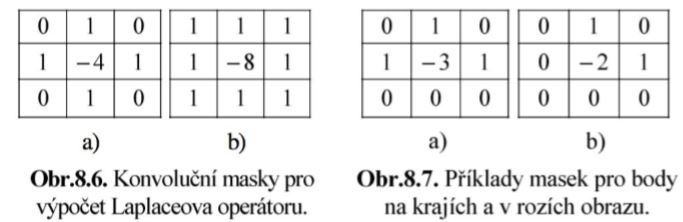
\includegraphics[width=0.5\textwidth]{assets/8_priklady_laplace}
	\end{center}
	\end{figure}
	\item Hrana je detekována jako \textbf{změna znaménka v průchodu mezi dvěma extrémy}.
	\item Je \textbf{více citlivý na šum než první derivace} (i při malém šumu je detekováno množství falešných hran).
	\item Pro redukci šumu a zahlazení vysokých frekvencí lze použít \textbf{Gaussův operátor}:
			\begin{equation*}
	 			\begin{bmatrix}
     			 1 &  2  &  1      \\[0.3em]
     			 2 &  1  &  2      \\[0.3em]
     			 1 &  2  &  1      \\
     			\end{bmatrix}.
			\end{equation*}
\end{itemize}
\subsubsection{Cannyho detekce hran}
Canny první stanovil požadavky, které by měl detektor splňovat a následně navrhl detektor. %zabili kennyho, parchanti
Požadavky:
\begin{itemize}
	\item \textbf{Minimalizovat} pravděpodobnost \textbf{chybné detekce}.
	\item Najít polohu hrany, co \textbf{nejpřesněji}.
	\item Bod hrany identifikovat \textbf{jednoznačně}.
\end{itemize}
\textbf{Postup:}
\begin{enumerate}
	\item Eliminace šumu Gaussovým filtrem.
	\item Velikost a směr gradientu -- nejčastěji Sobelův operátor (nebo centrální derivace).
	\item Nalezení lokálních maxim a stanovení interpolace v osmi okolí. \textbf{Redukce na hranu velikosti 1 px}.
	\item Eliminace nevýznamných hran (\textbf{double thresholding})
	\begin{itemize}
		\item Všechny body, kde je velikost hrany $\leq t_{high}$ -- \uv{jistá} hrana
		\item Pak ty, které jsou $ > t_{low}$ a sousedí s hranou -- \uv{jistá} hrana
	\end{itemize}
\end{enumerate}

%\subsection{Filtrace}
%\begin{itemize}
%	\item nic pořádného k segmentaci - filtraci jsem nenašel
%\end{itemize}